\documentclass{beamer}
\usecolortheme{dove}
\setbeamertemplate{navigation symbols}{}
\newenvironment{alltt}{\ttfamily}{\par}
\usepackage{amsmath,amssymb,amsfonts,amsthm, multicol, subfigure, color}
\usepackage{bm}
\usepackage{graphicx}
\usepackage{tabularx}
\usepackage{booktabs}
\usepackage{hyperref}
\usepackage{pdfpages}
\usepackage{xcolor}
\definecolor{dodgerblue}{rgb}{.118, .575, 1}
\definecolor{seagreen4}{RGB}{46, 139, 87}
\def\independenT#1#2{\mathrel{\rlap{$#1#2$}\mkern2mu{#1#2}}}
\newcommand\independent{\protect\mathpalette{\protect\independenT}{\perp}}
\newcommand\indep{\protect\mathpalette{\protect\independenT}{\perp}}
\def\logit{\text{logit}}
\usepackage{stackrel}
\usepackage{tikz}
\usetikzlibrary{arrows,shapes.arrows,positioning,shapes,patterns,calc}
\newcommand\slideref[1]{\vskip .1cm \scriptsize \textcolor{gray}{{#1}}}
\definecolor{seagreen}{RGB}{46, 139, 87}
\newcommand\red[1]{\color{red}#1}
\newcommand\blue[1]{\color{blue}#1}
\newcommand\gray[1]{\color{gray}#1}
\newcommand\green[1]{\color{olive}#1}
\newcommand\seagreen[1]{\color{seagreen}#1}
\newcommand\purple[1]{\color{purple}#1}
\newcommand\orange[1]{\color{orange}#1}
\newcommand\black[1]{\color{black}#1}
\newcommand\white[1]{\color{white}#1}
\newcommand\teal[1]{\color{teal}#1}
\newcommand\magenta[1]{\color{magenta}#1}
\newcommand\Fuchsia[1]{\color{Fuchsia}#1}
\newcommand\BlueGreen[1]{\color{BlueGreen}#1}
\newcommand\bblue[1]{\textcolor{blue}{\textbf{#1}}}
\newcommand\bred[1]{\textcolor{red}{\textbf{#1}}}
\newcommand\bgray[1]{\textcolor{gray}{\textbf{#1}}}
\newcommand\bgreen[1]{\textcolor{seagreen}{\textbf{#1}}}
\colorlet{lightgray}{gray!40}
\pgfdeclarelayer{bg}    % declare background layer for tikz
\pgfsetlayers{bg,main} % order layers for tikz
\newcommand\bref[2]{\href{#1}{\color{blue}{#2}}}
\newcommand\mycite[1]{\begin{scriptsize}\textcolor{darkgray}{(#1)}\end{scriptsize}}
\newcommand\iid{\stackrel{\text{iid}}{\sim}}
\newcommand\E{\text{E}}
\newcommand\V{\text{V}}
\renewcommand\P{\text{P}}
\newcommand{\Cov}{\text{Cov}}
\newcommand{\Cor}{\text{Cor}}
\newcommand\doop{\text{do}}
\newcommand{\tcframe}{\frame{
\small{
\only<1|handout:0>{\tableofcontents}
\only<2|handout:1>{\tableofcontents[currentsection]}}
}}
% Credit for the following to https://tex.stackexchange.com/questions/44983/beamer-removing-headline-and-its-space-on-a-single-frame-for-plan-but-keepin
\makeatletter
    \newenvironment{withoutheadline}{
        \setbeamertemplate{headline}[default]
        \def\beamer@entrycode{\vspace*{-\headheight}}
    }{}
\makeatother
\setbeamercovered{invisible}
\usepackage[round]{natbib}
\bibliographystyle{humannat-mod}
\setbeamertemplate{enumerate items}[default]
\usepackage{mathtools}
% BELOW THREE LINES MAKES NAME IN FOOTER
%\setbeamertemplate{footline}[text line]{%
%\parbox{\linewidth}{\vspace*{-8pt}Lundberg, Johnson, and Stewart. What is Your Estimand?}}%\hfill\insertshortauthor\hfill\insertpagenumber}}

%\setbeamertemplate{footline}[text line]{%
%\parbox{\linewidth}{\vspace*{-8pt}Ian Lundberg (Princeton)}}%\hfill\insertshortauthor\hfill\insertpagenumber}}
%t\setbeamertemplate{navigation symbols}{}

% Make the header figure that will appear frequently
\newcommand\headerfigure{
\begin{tikzpicture}[x = \textwidth, y = \textheight, every node/.style={anchor = center}]
\node at (0,1) {\resizebox{\textwidth}{!}{\begin{tikzpicture}[x = 1.7in, y = .3in]
    \node[cloud, draw, align=center, cloud puffs=20,cloud puff arc=110, aspect=2, inner sep=.5mm, font = \small] (general) at (-.1,0) {Theory or\\general goal};
    %%%%%%%%%%
    \node[align=center, font = \small] (theoretical) at (1,0) {Theoretical\\estimand};
    \draw[->, thick] (general) -- (theoretical);
    \node[align = center, anchor = south, font = {\bf\small}] at (.5,0) {Set};
    \node[align = center, anchor = north, font = \small] at (.5,0) {by argument};
    %%%%%%%%%%
    \node[align=center, font = \small] (empirical) at (2,0) {Empirical\\estimand};
    \draw[->, thick] (theoretical) -- (empirical);
    \node[align = center, anchor = south, font = {\bf\small}] at (1.5,0) {Link};
    \node[align = center, anchor = north, font = \small] at (1.5,0) {by assumption};
    %%%%%%%%%%
    \node[align=center, font = \small] (estimate) at (3,0) {Estimation\\strategy};
    \draw[->, thick] (empirical) -- (estimate);
    \node[align = center, anchor = south, font = {\bf\small}] at (2.5,0) {Learn};
    \node[align = center, anchor = north, font = \small] at (2.5,0) {by data};
    \end{tikzpicture}
    }};
\end{tikzpicture}
}
% Make the versions that have only one step in black
\newcommand\headerfigureset{
\begin{tikzpicture}[x = \textwidth, y = \textheight, every node/.style={anchor = center}]
\node at (0,1) {\resizebox{\textwidth}{!}{\begin{tikzpicture}[x = 1.7in, y = .3in]
    \node[cloud, draw, align=center, cloud puffs=20,cloud puff arc=110, aspect=2, inner sep=.5mm, font = \small] (general) at (-.1,0) {Theory or\\general goal};
    %%%%%%%%%%
    \node[align=center, font = \small] (theoretical) at (1,0) {Theoretical\\estimand};
    \draw[->, thick] (general) -- (theoretical);
    \node[align = center, anchor = south, font = {\bf\small}] at (.5,0) {Set};
    \node[align = center, anchor = north, font = \small] at (.5,0) {by argument};
    %%%%%%%%%%
    \node[align=center, font = \small, gray] (empirical) at (2,0) {Empirical\\estimand};
    \draw[->, thick, gray] (theoretical) -- (empirical);
    \node[align = center, anchor = south, font = {\bf\small}, gray] at (1.5,0) {Link};
    \node[align = center, anchor = north, font = \small, gray] at (1.5,0) {by assumption};
    %%%%%%%%%%
    \node[align=center, font = \small, gray] (estimate) at (3,0) {Estimation\\strategy};
    \draw[->, thick, gray] (empirical) -- (estimate);
    \node[align = center, anchor = south, font = {\bf\small}, gray] at (2.5,0) {Learn};
    \node[align = center, anchor = north, font = \small, gray] at (2.5,0) {by data};
    \end{tikzpicture}
    }};
\end{tikzpicture}
}
\newcommand\headerfigurelink{
\begin{tikzpicture}[x = \textwidth, y = \textheight, every node/.style={anchor = center}]
\node at (0,1) {\resizebox{\textwidth}{!}{\begin{tikzpicture}[x = 1.7in, y = .3in]
    \node[cloud, draw, align=center, cloud puffs=20,cloud puff arc=110, aspect=2, inner sep=.5mm, font = \small, gray] (general) at (-.1,0) {Theory or\\general goal};
    %%%%%%%%%%
    \node[align=center, font = \small] (theoretical) at (1,0) {Theoretical\\estimand};
    \draw[->, thick, gray] (general) -- (theoretical);
    \node[align = center, anchor = south, font = {\bf\small}, gray] at (.5,0) {Set};
    \node[align = center, anchor = north, font = \small, gray] at (.5,0) {by argument};
    %%%%%%%%%%
    \node[align=center, font = \small] (empirical) at (2,0) {Empirical\\estimand};
    \draw[->, thick] (theoretical) -- (empirical);
    \node[align = center, anchor = south, font = {\bf\small}] at (1.5,0) {Link};
    \node[align = center, anchor = north, font = \small] at (1.5,0) {by assumption};
    %%%%%%%%%%
    \node[align=center, font = \small, gray] (estimate) at (3,0) {Estimation\\strategy};
    \draw[->, thick, gray] (empirical) -- (estimate);
    \node[align = center, anchor = south, font = {\bf\small}, gray] at (2.5,0) {Learn};
    \node[align = center, anchor = north, font = \small, gray] at (2.5,0) {by data};
    \end{tikzpicture}
    }};
\end{tikzpicture}
}
\newcommand\headerfigurelearn{
\begin{tikzpicture}[x = \textwidth, y = \textheight, every node/.style={anchor = center}]
\node at (0,1) {\resizebox{\textwidth}{!}{\begin{tikzpicture}[x = 1.7in, y = .3in]
    \node[cloud, draw, align=center, cloud puffs=20,cloud puff arc=110, aspect=2, inner sep=.5mm, font = \small, gray] (general) at (-.1,0) {Theory or\\general goal};
    %%%%%%%%%%
    \node[align=center, font = \small, gray] (theoretical) at (1,0) {Theoretical\\estimand};
    \draw[->, thick, gray] (general) -- (theoretical);
    \node[align = center, anchor = south, font = {\bf\small}, gray] at (.5,0) {Set};
    \node[align = center, anchor = north, font = \small, gray] at (.5,0) {by argument};
    %%%%%%%%%%
    \node[align=center, font = \small] (empirical) at (2,0) {Empirical\\estimand};
    \draw[->, thick, gray] (theoretical) -- (empirical);
    \node[align = center, anchor = south, font = {\bf\small}, gray] at (1.5,0) {Link};
    \node[align = center, anchor = north, font = \small, gray] at (1.5,0) {by assumption};
    %%%%%%%%%%
    \node[align=center, font = \small] (estimate) at (3,0) {Estimation\\strategy};
    \draw[->, thick] (empirical) -- (estimate);
    \node[align = center, anchor = south, font = {\bf\small}] at (2.5,0) {Learn};
    \node[align = center, anchor = north, font = \small] at (2.5,0) {by data};
    \end{tikzpicture}
    }};
\end{tikzpicture}
}

\newcommand\estimandFigure{

\begin{tikzpicture}[x = \textwidth, y = \textheight, every node/.style={anchor = center}]
%\node at (0,1) {\resizebox{\textwidth}{!}{\begin{tikzpicture}[x = 1.7in, y = .3in]
\node<10->[circle, fill = lightgray, draw = lightgray, font = \footnotesize, inner sep = 8pt] (point1) at (.18,.55) {};
\node<10->[gray, font = \footnotesize, align = center, anchor = north] (usqNote) at (point1.south) {A \bgray{unit-specific}\\\bgray{quantity}};
\node[circle, fill = lightgray, draw = lightgray, font = \footnotesize, inner sep = 8pt] (point2) at (.33,.5) {};
\node[circle, fill = lightgray, draw = lightgray, font = \footnotesize, inner sep = 8pt] (point3) at (.25,.35) {};
\node[circle, fill = lightgray, draw = lightgray, font = \footnotesize, inner sep = 8pt] (point4) at (.4,.38) {};
\node[circle, fill = lightgray, draw = lightgray, font = \footnotesize, inner sep = 8pt] (point5) at (.12,.37) {};
\node[circle, fill = lightgray, draw = lightgray, font = \footnotesize, inner sep = 8pt] (point6) at (.45,.55) {};
\draw[line width = 2pt, gray, rounded corners] (.05,.3) rectangle (.5,.6);
\node[gray, font = \footnotesize, align = left, anchor = south west] at (.5,.3) {Averaged over a\\\bgray{target population}};
\node[font = \scriptsize] at (point1) {$Y_i(t)$};
\node[font = \scriptsize] at (point2) {$Y_i(t)$};
\node[font = \scriptsize] at (point3) {$Y_i(t)$};
\node[font = \scriptsize] at (point4) {$Y_i(t)$};
\node[font = \scriptsize] at (point5) {$Y_i(t)$};
\node[font = \scriptsize] at (point6) {$Y_i(t)$};
    \end{tikzpicture}
    %}};
%\end{tikzpicture}
}

\newcommand\estimandFigureBottomCaption{

\begin{tikzpicture}[x = \textwidth, y = \textheight, every node/.style={anchor = center}]
%\node at (0,1) {\resizebox{\textwidth}{!}{\begin{tikzpicture}[x = 1.7in, y = .3in]
\node[circle, fill = lightgray, draw = lightgray, font = \footnotesize, inner sep = 8pt] (point1) at (.18,.55) {};
\node[gray, font = \footnotesize, align = center, anchor = north] (usqNote) at (point1.south) {A \bgray{unit-specific}\\\bgray{quantity}};
\node[circle, fill = lightgray, draw = lightgray, font = \footnotesize, inner sep = 8pt] (point2) at (.33,.5) {};
\node[circle, fill = lightgray, draw = lightgray, font = \footnotesize, inner sep = 8pt] (point3) at (.25,.35) {};
\node[circle, fill = lightgray, draw = lightgray, font = \footnotesize, inner sep = 8pt] (point4) at (.4,.38) {};
\node[circle, fill = lightgray, draw = lightgray, font = \footnotesize, inner sep = 8pt] (point5) at (.12,.37) {};
\node[circle, fill = lightgray, draw = lightgray, font = \footnotesize, inner sep = 8pt] (point6) at (.45,.55) {};
\draw[line width = 2pt, gray, rounded corners] (.05,.3) rectangle (.5,.6);
\node[gray, font = \footnotesize, align = center, anchor = north] at (.275,.3) {Averaged over a\\\bgray{target population}};
\node[font = \scriptsize] at (point1) {$Y_i(t)$};
\node[font = \scriptsize] at (point2) {$Y_i(t)$};
\node[font = \scriptsize] at (point3) {$Y_i(t)$};
\node[font = \scriptsize] at (point4) {$Y_i(t)$};
\node[font = \scriptsize] at (point5) {$Y_i(t)$};
\node[font = \scriptsize] at (point6) {$Y_i(t)$};
    \end{tikzpicture}
    %}};
%\end{tikzpicture}
}

\newcommand\estimandFigureBottomCaptionCustom[5]{
\begin{tikzpicture}[x = #4\textwidth, y = #5\textheight, every node/.style={anchor = center}]
\node[circle, fill = lightgray, draw = lightgray, font = \footnotesize, inner sep = #3] (point1) at (.18,.55) {};
\node[gray, font = \footnotesize, align = center, anchor = north] (usqNote) at (point1.south) {A \bgray{unit-specific}\\\bgray{quantity}};
\node[circle, fill = lightgray, draw = lightgray, font = \footnotesize, inner sep = #3] (point2) at (.41,.5) {};
\node[circle, fill = lightgray, draw = lightgray, font = \footnotesize, inner sep = #3] (point3) at (.25,.35) {};
\node[circle, fill = lightgray, draw = lightgray, font = \footnotesize, inner sep = #3] (point4) at (.4,.38) {};
\node[circle, fill = lightgray, draw = lightgray, font = \footnotesize, inner sep = #3] (point5) at (.12,.37) {};
\draw[line width = 2pt, gray, rounded corners] (.05,.3) rectangle (.5,.6);
\node[gray, font = \footnotesize, align = center, anchor = north] at (.275,.3) {Averaged over a\\\bgray{target population}};
\node[font = #2, align = left] at (point1) {#1};
\node[font = #2, align = left] at (point2) {#1};
\node[font = #2, align = left] at (point3) {#1};
\node[font = #2, align = left] at (point4) {#1};
\node[font = #2, align = left] at (point5) {#1};
    \end{tikzpicture}
}

\newcommand\estimandFigureBottomCaptionCustomDiamond[5]{
\begin{tikzpicture}[x = #4\textwidth, y = #5\textheight, every node/.style={anchor = center}]
\node[diamond, fill = lightgray, draw = lightgray, font = \footnotesize, inner sep = #3] (point1) at (.18,.55) {};
\node[gray, font = \footnotesize, align = center, anchor = north] (usqNote) at (point1.south) {A \bgray{unit-specific}\\\bgray{quantity}};
\node[diamond, fill = lightgray, draw = lightgray, font = \footnotesize, inner sep = #3] (point2) at (.41,.5) {};
\node[diamond, fill = lightgray, draw = lightgray, font = \footnotesize, inner sep = #3] (point3) at (.25,.35) {};
\node[diamond, fill = lightgray, draw = lightgray, font = \footnotesize, inner sep = #3] (point4) at (.4,.38) {};
\node[diamond, fill = lightgray, draw = lightgray, font = \footnotesize, inner sep = #3] (point5) at (.12,.37) {};
\draw[line width = 2pt, gray, rounded corners] (.05,.3) rectangle (.5,.6);
\node[gray, font = \footnotesize, align = center, anchor = north] at (.275,.3) {Averaged over a\\\bgray{target population}};
\node[font = #2, align = left] at (point1) {#1};
\node[font = #2, align = left] at (point2) {#1};
\node[font = #2, align = left] at (point3) {#1};
\node[font = #2, align = left] at (point4) {#1};
\node[font = #2, align = left] at (point5) {#1};
    \end{tikzpicture}
}

\newcommand\estimandFigureBottomCaptionCustomPager[6]{
\begin{tikzpicture}[x = #4\textwidth, y = #5\textheight, every node/.style={anchor = center}]
\node[circle, fill = lightgray, draw = lightgray, font = \footnotesize, inner sep = #3] (point1) at (.18,.53) {};
\node[gray, font = \footnotesize, align = center, anchor = north] (usqNote) at (point1.south) {A \bgray{unit-specific}\\\bgray{quantity}};
\node[circle, fill = lightgray, draw = lightgray, font = \footnotesize, inner sep = #3] (point2) at (.4,.5) {};
\node[circle, fill = lightgray, draw = lightgray, font = \footnotesize, inner sep = #3] (point3) at (.32,.38) {};
\draw[line width = 2pt, gray, rounded corners] (.05,.3) rectangle (.5,.6);
\node[gray, font = \footnotesize, align = center, anchor = north] at (.275,.3) {#6};
\node[font = #2, align = left] at (point1) {#1};
\node[font = #2, align = left] at (point2) {#1};
\node[font = #2, align = left] at (point3) {#1};
    \end{tikzpicture}
}

\newcommand\estimandFigureBottomCaptionCustomPagerWhite[6]{
\begin{tikzpicture}[x = #4\textwidth, y = #5\textheight, every node/.style={anchor = center}]
\node[ellipse, fill = lightgray, draw = lightgray, font = \footnotesize] (point1) at (.31,.56) {$Y_i(\text{No record})$};
\node[gray, font = \footnotesize, align = center, anchor = north] (usqNote) at (point1.south) {A \bgray{unit-specific}\\\bgray{quantity}};
\node[ellipse, fill = lightgray, draw = lightgray, font = \footnotesize] (point2) at (.24,.43) {$Y_i(\text{No record})$};
\node[ellipse, fill = lightgray, draw = lightgray, font = \footnotesize] (point3) at (.31,.35) {$Y_i(\text{No record})$};
\draw[line width = 2pt, gray, rounded corners] (.05,.3) rectangle (.5,.6);
\node[gray, font = \footnotesize, align = center, anchor = north] at (.275,.3) {#6};
    \end{tikzpicture}
}

\newcommand\estimandFigureBottomCaptionCustomPagerBlack[6]{
\begin{tikzpicture}[x = #4\textwidth, y = #5\textheight, every node/.style={anchor = center}]
\node[rounded corners, fill = lightgray, draw = lightgray, font = \footnotesize] (point1) at (.24,.56) {$Y_i(\text{No record})$};
\node[gray, font = \footnotesize, align = center, anchor = north] (usqNote) at (point1.south) {A \bgray{unit-specific}\\\bgray{quantity}};
\node[rounded corners, fill = lightgray, draw = lightgray, font = \footnotesize] (point2) at (.31,.43) {$Y_i(\text{No record})$};
\node[rounded corners, fill = lightgray, draw = lightgray, font = \footnotesize] (point3) at (.24,.35) {$Y_i(\text{No record})$};
\draw[line width = 2pt, gray, rounded corners] (.05,.3) rectangle (.5,.6);
\node[gray, font = \footnotesize, align = center, anchor = north] at (.275,.3) {#6};
\end{tikzpicture}
}

\newcommand\estimandFigureNoCaptionCustom[5]{
\begin{tikzpicture}[x = #4\textwidth, y = #5\textheight, every node/.style={anchor = center}]
\node[circle, fill = lightgray, draw = lightgray, font = \footnotesize, inner sep = #3] (point1) at (.18,.53) {};
%\node[gray, font = \footnotesize, align = center, anchor = north] (usqNote) at (point1.south) {A \bgray{unit-specific}\\\bgray{quantity}};
\node[circle, fill = lightgray, draw = lightgray, font = \footnotesize, inner sep = #3] (point2) at (.41,.5) {};
\node[circle, fill = lightgray, draw = lightgray, font = \footnotesize, inner sep = #3] (point3) at (.25,.4) {};
\node[circle, fill = lightgray, draw = lightgray, font = \footnotesize, inner sep = #3] (point4) at (.4,.38) {};
\node[circle, fill = lightgray, draw = lightgray, font = \footnotesize, inner sep = #3] (point5) at (.12,.37) {};
\draw[line width = 2pt, gray, rounded corners] (.05,.3) rectangle (.5,.6);
%\node[gray, font = \footnotesize, align = center, anchor = north] at (.275,.3) {Averaged over a\\\bgray{target population}};
\node[font = #2, align = left] at (point1) {#1};
\node[font = #2, align = left] at (point2) {#1};
\node[font = #2, align = left] at (point3) {#1};
\node[font = #2, align = left] at (point4) {#1};
\node[font = #2, align = left] at (point5) {#1};
    \end{tikzpicture}
}

\newcommand\estimandFigureNoCaptionMissingA[5]{
\begin{tikzpicture}[x = #4\textwidth, y = #5\textheight, every node/.style={anchor = center}]
\node[circle, fill = lightgray, draw = black, line width = 1.3pt, font = \footnotesize, inner sep = #3] (point1) at (.18,.53) {};
\node[circle, fill = lightgray, draw = black, line width = 1.3pt, font = \footnotesize, inner sep = #3] (point2) at (.41,.5) {};
\node[circle, fill = lightgray, draw = black, line width = 1.3pt, font = \footnotesize, inner sep = #3] (point3) at (.25,.4) {};
\node[circle, fill = lightgray, draw = lightgray, font = \footnotesize, inner sep = #3] (point4) at (.4,.38) {};
\node[circle, fill = lightgray, draw = lightgray, font = \footnotesize, inner sep = #3] (point5) at (.12,.37) {};
\draw[line width = 2pt, gray, rounded corners] (.05,.3) rectangle (.5,.6);
%\node[gray, font = \footnotesize, align = center, anchor = north] at (.275,.3) {Averaged over a\\\bgray{target population}};
\node[font = #2, align = left] at (point1) {#1};
\node[font = #2, align = left] at (point2) {#1};
\node[font = #2, align = left] at (point3) {#1};
\node[font = #2, align = left] at (point4) {#1};
\node[font = #2, align = left] at (point5) {#1};
    \end{tikzpicture}
}

\newcommand\estimandFigureNoCaptionMissingB[5]{
\begin{tikzpicture}[x = #4\textwidth, y = #5\textheight, every node/.style={anchor = center}]
\node[circle, fill = lightgray, draw = lightgray, font = \footnotesize, inner sep = #3] (point1) at (.18,.53) {};
\node[circle, fill = lightgray, draw = lightgray, font = \footnotesize, inner sep = #3] (point2) at (.41,.5) {};
\node[circle, fill = lightgray, draw = lightgray, font = \footnotesize, inner sep = #3] (point3) at (.25,.4) {};
\node[circle, fill = lightgray, draw = black, line width = 1.3pt, font = \footnotesize, inner sep = #3] (point4) at (.4,.38) {};
\node[circle, fill = lightgray, draw = black, line width = 1.3pt, font = \footnotesize, inner sep = #3] (point5) at (.12,.37) {};
\draw[line width = 2pt, gray, rounded corners] (.05,.3) rectangle (.5,.6);
\node[font = #2, align = left] at (point1) {#1};
\node[font = #2, align = left] at (point2) {#1};
\node[font = #2, align = left] at (point3) {#1};
\node[font = #2, align = left] at (point4) {#1};
\node[font = #2, align = left] at (point5) {#1};
    \end{tikzpicture}
}

\newcommand\estimandFigureNoCaptionImputedA[5]{
\begin{tikzpicture}[x = #4\textwidth, y = #5\textheight, every node/.style={anchor = center}]
\node[circle, fill = lightgray, draw = black, line width = 1.3pt, font = \footnotesize, inner sep = #3] (point1) at (.18,.53) {};
\node[circle, fill = lightgray, draw = black, line width = 1.3pt, font = \footnotesize, inner sep = #3] (point2) at (.41,.5) {};
\node[circle, fill = lightgray, draw = black, line width = 1.3pt, font = \footnotesize, inner sep = #3] (point3) at (.25,.4) {};
\node[circle, fill = lightgray, draw = lightgray, font = \footnotesize, inner sep = #3] (point4) at (.4,.38) {};
\node[circle, fill = lightgray, draw = lightgray, font = \footnotesize, inner sep = #3] (point5) at (.12,.37) {};
\draw[line width = 2pt, gray, rounded corners] (.05,.3) rectangle (.5,.6);
%\node[gray, font = \footnotesize, align = center, anchor = north] at (.275,.3) {Averaged over a\\\bgray{target population}};
\node[font = #2, align = left] at (point1) {$Y_i(1)$};
\node[font = #2, align = left] at (point2) {$Y_i(1)$};
\node[font = #2, align = left] at (point3) {$Y_i(1)$};
\node[font = #2, align = left] at (point4) {$\hat{Y}_i(1)$};
\node[font = #2, align = left] at (point5) {$\hat{Y}_i(1)$};
    \end{tikzpicture}
}

\newcommand\estimandFigureNoCaptionImputedB[5]{
\begin{tikzpicture}[x = #4\textwidth, y = #5\textheight, every node/.style={anchor = center}]
\node[circle, fill = lightgray, draw = lightgray, font = \footnotesize, inner sep = #3] (point1) at (.18,.53) {};
\node[circle, fill = lightgray, draw = lightgray, font = \footnotesize, inner sep = #3] (point2) at (.41,.5) {};
\node[circle, fill = lightgray, draw = lightgray, font = \footnotesize, inner sep = #3] (point3) at (.25,.4) {};
\node[circle, fill = lightgray, draw = black, line width = 1.3pt, font = \footnotesize, inner sep = #3] (point4) at (.4,.38) {};
\node[circle, fill = lightgray, draw = black, line width = 1.3pt, font = \footnotesize, inner sep = #3] (point5) at (.12,.37) {};
\draw[line width = 2pt, gray, rounded corners] (.05,.3) rectangle (.5,.6);
\node[font = #2, align = left] at (point1) {$\hat{Y}_i(0)$};
\node[font = #2, align = left] at (point2) {$\hat{Y}_i(0)$};
\node[font = #2, align = left] at (point3) {$\hat{Y}_i(0)$};
\node[font = #2, align = left] at (point4) {$Y_i(0)$};
\node[font = #2, align = left] at (point5) {$Y_i(0)$};
    \end{tikzpicture}
}

\newcommand\estimandFigureSideCaptionCustom[5]{
\begin{tikzpicture}[x = #4\textwidth, y = #5\textheight, every node/.style={anchor = center}]
\node[circle, fill = lightgray, draw = lightgray, font = \footnotesize, inner sep = #3] (point1) at (.18,.48) {};
\node[gray, font = \footnotesize, align = center, anchor = north] (usqNote) at (point1.south) {A \bgray{unit-specific}\\\bgray{quantity}};
\node[circle, fill = lightgray, draw = lightgray, font = \footnotesize, inner sep = #3] (point2) at (.41,.53) {};
%\node[circle, fill = lightgray, draw = lightgray, font = \footnotesize, inner sep = #3] (point3) at (.25,.35) {};
\node[circle, fill = lightgray, draw = lightgray, font = \footnotesize, inner sep = #3] (point4) at (.38,.38) {};
%\node[circle, fill = lightgray, draw = lightgray, font = \footnotesize, inner sep = #3] (point5) at (.12,.37) {};
\draw[line width = 2pt, gray, rounded corners] (.05,.3) rectangle (.5,.6);
\node[gray, font = \footnotesize, align = left, anchor = south west] at (.5,.3) {Averaged over a\\\bgray{target population}};
\node[font = #2, align = left] at (point1) {#1};
\node[font = #2, align = left] at (point2) {#1};
%\node[font = #2, align = left] at (point3) {#1};
\node[font = #2, align = left] at (point4) {#1};
%\node[font = #2, align = left] at (point5) {#1};
    \end{tikzpicture}
}


\title{What is Your Estimand}
\author{Lundberg, Johnson, Stewart}
\date{\today}

\begin{document}

\begin{frame}
\centering
\begin{tikzpicture}[x = .5\textwidth, y = .5\textwidth]
\node at (-1,-1) {};
\node at (1,1) {};
\node[font = \LARGE, align = left, anchor = north west, blue] at (-1, .9) {\textbf{What is Your Estimand?}};
\node[font = \LARGE, align = left, anchor = north west] at (-1,.7) {A workshop on\\specifying quantitative\\research goals};
\node[anchor = north east] at (1,1) {
\includegraphics[width = 1.3in]{output/target}};
%\node[anchor = north east] at (1, .9) {4 August 2020};
%\node[anchor = north east, align = right] at (1, .8) {Annual Meeting of the\\American Sociological\\Association};
\node[align = center, anchor = south east, align = left] (ian) at (-.56, .05) {Ian Lundberg};
\node[align = center, anchor = south] (rebecca) at (-.13,.05) {Rebecca Johnson};
\node[align = center, anchor = south west] (brandon) at (.3, .05) {Brandon M. Stewart};
\node[align = center, anchor = north, font = \scriptsize] (ianAffil) at (ian.south) {UCLA\\Sociology\\\bref{https://www.ianlundberg.org/}{ianlundberg.org}};%\\ilundberg@princeton.edu};
\node[align = center, anchor = north, font = \scriptsize] (rebeccaAffil) at (rebecca.south) {Dartmouth Quantitative\\Social Science\\\bref{https://www.rebeccajohnson.io/}{rebeccajohnson.io}};%\\rebecca.ann.johnson\\@dartmouth.edu};
\node[align = center, anchor = north, font = \scriptsize] (brandonAffil) at (brandon.south) {Princeton\\Sociology\\\bref{http://scholar.princeton.edu/bstewart}{brandonstewart.org}};%\\bms4@princeton.edu};
\node[align = left, anchor = south west, font = \scriptsize, text width = \textwidth] at (-1, -.33) {\textbf{NOTE:} These slides are for a pedagogical workshop.\\The main slides for this paper are \bref{https://github.com/ilundberg/slides/blob/master/what_is_your_estimand/what_is_your_estimand_cornell_csi.pdf}{here}.};
\node[align = left, anchor = south west, font = \scriptsize, text width = \textwidth] at (-1, -.65) {15 October 2021. Cornell Population Center Training Workshop. \\Paper in \emph{American Sociological Review}. Preprint on \bref{https://doi.org/10.31235/osf.io/ba67n}{SocArxiv}. Replication code on  \bref{https://doi.org/10.7910/DVN/ASGOVU}{Dataverse}. Research reported in this publication was supported by The Eunice Kennedy Shriver National Institute of Child Health \& Human Development of the National Institutes of Health under Award Number P2CHD047879.};
\end{tikzpicture}
\end{frame}

\begin{frame}{Plan for today}
\begin{itemize}
\item Brief recap of paper: ``What is Your Estimand?''
\item In groups, we will discuss
\begin{itemize}
\item Defining the intervention in a causal estimand
\item Defining the target population in a descriptive estimand
\item Policy implications of descriptive and causal estimands
\end{itemize}
\item Professional development: Open for questions
\end{itemize}
\end{frame}

\section{Intro}

\begin{frame}{Research framework: Estimands connect theory to evidence}
{\begin{tikzpicture}[x = 1.1in, y = .3in]
    \node[cloud, draw, align=center, cloud puffs=20,cloud puff arc=110, aspect=2, inner sep=.5mm] (general) at (-.2,0) {Theory or\\general goal};
    \node[align=center, white] (theoretical) at (1,0) {Theoretical\\estimand};
    \node[align=center, white] (empirical) at (2,0) {Empirical\\estimand};
    \node[align=center] (estimate) at (3,0) {Estimation\\strategy};
    \draw[->, thick] (general) -- (theoretical);
    \draw[->, thick] (theoretical) -- (empirical);
    \draw[->, thick] (empirical) -- (estimate);
    %%%%%%%%%%
 \node<2-4>[anchor = north, align = center, font = {\bf\footnotesize}, seagreen] at (-.2,-2) {Pages of theory};
 \draw<2-4>[->, seagreen, line width = 1.5pt] (-.2,-2) -- (.-.2,-1.2);
 \node<3-4>[anchor = north, align = center, font = {\bf\footnotesize}, seagreen] at (3,-2) {Pages of things\\done to data};
 \draw<3-4>[->, seagreen, line width = 1.5pt] (3,-2) -- (3,-1.2);
 \node<4>[anchor = north, align = center, font = {\bf\footnotesize}, red] at (1.5,-2) {Nothing in between};
 \draw<4>[->, red, line width = 1.5pt] (1.3,-2) -- (1.1,-1.2);
 \draw<4>[->, red, line width = 1.5pt] (1.7,-2) -- (1.9,-1.2);
    %%%%%%%%%%
    \node<5->[align=center] (theoretical) at (1,0) {Theoretical\\estimand};
    \node<6->[align=center, font = \footnotesize, anchor = north] (define) at (.5,-1) {\textbf{Set}\\a specific\\target};
    %\node[align=center, font = \scriptsize, anchor = north west] at (-.6,-5.4) {\textbf{Example tools:}};
    %\node[align=center, font = \scriptsize, anchor = north] at (.5,-5.4) {Target population,\\Causal contrast};
    \draw<6->[->, thick] (define) -- (.5,-.3);
    %\draw[thick] (.5,-5.3) -- (.5,-4.5);
    \draw<7-17>[line width = 2pt, gray] (-.5,-3.5) -- node[midway, above, text = black] {Definition} (.5,-3.5);
     \node<7-11>[align = center, rounded corners, font = \footnotesize, anchor = north, text width = 1.1in] at (0, -3.7) {A \bblue{unit-specific quantity}\\aggregated over a\\\bblue{target population}};
    \draw<8-17>[line width = 2pt, gray] (.6,-3.5) -- node[midway, above, text = black] {Example} (3.5,-3.5);
     \node<8>[anchor = north west, font = \footnotesize] at (.6,-4) {$\begin{aligned}\frac{1}{\substack{\text{Size of U.S.}\\\text{adult population}}}\sum_{\substack{i\text{ in U.S.}\\\text{adult population}}}\bigg(\text{Employed}_i\bigg)\end{aligned}$};
     \node<9-10>[anchor = north west, font = \footnotesize] at (.6,-4) {$\begin{aligned}\frac{1}{\substack{\text{Size of U.S.}\\\text{adult population}}}\sum_{\substack{i\text{ in U.S.}\\\text{adult population}}} \bigg(&\underbrace{\text{Employed}_i(\text{Job training})}_{\substack{\text{Employment if received}\\\text{job training}}} \\ &- \underbrace{\text{Employed}_i(\text{No job training})}_{\substack{\text{Employment if did not receive}\\\text{job training}}}\bigg) \end{aligned}$};
    \node<10-11>[align=right, gray, font = \footnotesize, anchor = south east] (define) at (3.5,-9.5) {Lieberson 1987, Abbott 1988, Freedman 1991, Xie 2013, Hern\'an 2018};
     %\node<11>[anchor = north] at (2.05,-3.7) {\estimandFigureNoCaptionCustom{$Y_i(1)$\\$-Y_i(0)$}{\tiny}{6pt}{1}{.7}};
     \node<11-12>[anchor = north west] at (.8,-3.7) {\estimandFigureNoCaptionCustom{$Y_i(1)$}{\tiny}{6pt}{.5}{.7}};
     \draw<11-17>[line width = 1.2pt] (1.95,-5.3) -- (2.15,-5.3);
     \node<11-13>[anchor = north east] at (3.3,-3.7) {\estimandFigureNoCaptionCustom{$Y_i(0)$}{\tiny}{6pt}{.5}{.7}};
    %%%%%%%%%%
    \node<5->[align=center] (empirical) at (2,0) {Empirical\\estimand};
    \node<12->[align=center, font = \footnotesize, anchor = north] (identify) at (1.5,-1) {\textbf{Link}\\to observable\\data};
    %\node[align=center, font = \footnotesize, anchor = north] at (1.5,-5.4) {Directed Acyclic Graphs,\\Potential outcomes};
    \draw<12->[->, thick] (identify) -- (1.5,-.3);
     \node<12-15>[align = center, rounded corners, font = \footnotesize, anchor = north, text width = 1.1in] at (0, -3.7) {A quantity involving \bblue{observable data}};
     \node<13-16>[anchor = north west] at (.8,-3.7) {\estimandFigureNoCaptionMissingA{$Y_i(1)$}{\tiny}{6pt}{.5}{.7}};
     \node<14-16>[anchor = north east] at (3.3,-3.7) {\estimandFigureNoCaptionMissingB{$Y_i(0)$}{\tiny}{6pt}{.5}{.7}};
      \node<15> (x) at (1.5,-7.3) {$\vec{X}$};
      \node<15> (d) at (2,-7.3) {$T$};
      \node<15> (y) at (2.5,-7.3) {$Y$};
      \draw<15>[->, thick] (x) -- (d);
      \draw<15>[->, thick] (x) to[bend right] (y);
      \draw<15>[->, thick] (d) -- (y);
    \node<15>[align=right, gray, font = \footnotesize, anchor = south east] (define) at (3.5,-9.5) {Pearl 2009, Imbens and Rubin 2015,\\Morgan and Winship 2015, Elwert and Winship 2014};
    %%%%%%%%%%
    \node<16->[align=center, font = \footnotesize, anchor = north] (learn) at (2.5,-1) {\textbf{Learn}\\from data};
    %\node[align=center, font = \footnotesize, anchor = north] at (2.5,-5.4) {OLS regression,\\Machine learning};
    \draw<16->[->, thick] (learn) -- (2.5,-.3);
    %\draw[thick] (2.5,-5.3) -- (2.5,-4.5);
     \node<16-17>[align = center, rounded corners, font = \footnotesize, anchor = north, text width = 1.1in] at (0, -3.7) {An algorithm applied to data};
     \node<17>[anchor = north west] at (.8,-3.7) {\estimandFigureNoCaptionImputedA{$Y_i(1)$}{\tiny}{6pt}{.5}{.7}};
     \node<17>[anchor = north east] at (3.3,-3.7) {\estimandFigureNoCaptionImputedB{$Y_i(0)$}{\tiny}{6pt}{.5}{.7}};
    %\node<17-18>[anchor = north west, font = \scriptsize] at (.6,-3.7) {$\begin{aligned}\hat\theta &= \underbrace{\frac{1}{n}\sum_{i=1}^n}_{\substack{\text{Sample}\\\text{average}}} \bigg(\underbrace{\hat\E(Y\mid \vec{X} = \vec{x}_i, D = 1)}_{\substack{\text{Regression prediction}\\\text{if treated}}} - \underbrace{\hat\E(Y\mid \vec{X} = \vec{x}_i, D = 0)}_{\substack{\text{Regression prediction}\\\text{if untreated}}}\bigg)\end{aligned}$};
    \node<17>[align=right, gray, font = \footnotesize, anchor = south east] (define) at (3.5,-9.5) {Young 2009, Watts 2014, Berk et al. 2019, Molina and Garip 2019};
    % Types of argument
    \onslide<19->{
    \node[align=center, font = \footnotesize, anchor = north] at (.5,-3.7) {By argument};
    \draw[thick] (.5,-3.8) -- (.5,-2.8);
    \node[align=center, font = \footnotesize, anchor = north] at (1.5,-3.7) {By assumption};
    \draw[thick] (1.5,-3.8) -- (1.5,-2.8);
    \node[align=center, font = \footnotesize, anchor = north] at (2.5,-3.7) {By data};
    \draw[thick] (2.5,-3.8) -- (2.5,-2.8);
    }
    \end{tikzpicture}
    }
\end{frame}


% BEGIN WORKSHOP SLIDES

\section{Set}

\begin{frame}[t]\headerfigureset \vskip 1in
\huge 1. Set the target quantity.
\end{frame}

% DESCRIBE POPULATION
\begin{frame}[t]\headerfigureset
\begin{tikzpicture}[x = \textwidth, y = .8\textheight]
\node at (0,0) {};
\node at (1,1) {};
\node[anchor = west, font = {\large\bf}] (goal) at (0, .9) {Describe a population};
\draw[line width = 1.5pt, line cap = round] (goal.south west) -- (goal.south east);
\node[anchor = west] at (0, .75) {What is the proportion employed};
\node[anchor = west] at (0, .68) {among U.S. resident women ages 21--35?};
% Title rows
\only<2->{
\node[font = \footnotesize, anchor = east] at (.4, .4) {Woman 1};
\node[font = \footnotesize, anchor = east] at (.4, .35) {Woman 2};
\node[font = \footnotesize, anchor = east] at (.4, .3) {Woman 3};
\node[font = \footnotesize, anchor = east] at (.4, .25) {Woman 4};
}
\only<3->{
% Title columns
\node[font = \footnotesize, anchor = south] (emp) at (.5, .45) {Employed?};
\draw[thick] (.4,.45) -- (.6, .45);
% Cell values
\node[font = \footnotesize] at (.5, .4) {1};
\node[font = \footnotesize] at (.5, .35) {0};
\node[font = \footnotesize] at (.5, .3) {1};
\node[font = \footnotesize] at (.5, .25) {1};
}
\end{tikzpicture}
\end{frame}

% DESCRIBE POPULATION SUBGROUPS
\begin{frame}[t]\headerfigureset
\begin{tikzpicture}[x = \textwidth, y = .8\textheight]
\node at (0,0) {};
\node at (1,1) {};
\node[anchor = west, font = {\large\bf}] (goal) at (0, .9) {Describe population subgroups};
\draw[line width = 1.5pt, line cap = round] (goal.south west) -- (goal.south east);
\node[anchor = west] at (0, .75) {What is the proportion employed};
\node[anchor = west] at (0, .68) {among U.S. resident women ages 21--35,};
\node[anchor = west] at (0, .61) {comparing mothers to non-mothers?};
% MOTHERS
% Title rows
\only<2->{
\node[font = \footnotesize, anchor = east] at (.2, .4) {Mother 1};
\node[font = \footnotesize, anchor = east] at (.2, .35) {Mother 2};
\node[font = \footnotesize, anchor = east] at (.2, .3) {Mother 3};
\node[font = \footnotesize, anchor = east] at (.2, .25) {Mother 4};
% Title columns
\node[font = \footnotesize, anchor = south] (emp) at (.3, .45) {Employed?};
\draw[thick] (.2,.45) -- (.4, .45);
% Cell values
\node[font = \footnotesize] at (.3, .4) {0};
\node[font = \footnotesize] at (.3, .35) {0};
\node[font = \footnotesize] at (.3, .3) {0};
\node[font = \footnotesize] at (.3, .25) {1};
% NON-MOTHERS
% Title rows
\node[font = \footnotesize, anchor = east] at (.7, .4) {Non-Mother 1};
\node[font = \footnotesize, anchor = east] at (.7, .35) {Non-Mother 2};
\node[font = \footnotesize, anchor = east] at (.7, .3) {Non-Mother 3};
\node[font = \footnotesize, anchor = east] at (.7, .25) {Non-Mother 4};
% Title columns
\node[font = \footnotesize, anchor = south] (emp) at (.8, .45) {Employed?};
\draw[thick] (.7,.45) -- (.9, .45);
% Cell values
\node[font = \footnotesize] at (.8, .4) {1};
\node[font = \footnotesize] at (.8, .35) {0};
\node[font = \footnotesize] at (.8, .3) {1};
\node[font = \footnotesize] at (.8, .25) {1};
}
\end{tikzpicture}
\end{frame}

% CAUSAL EFFECT IN A POPULATION
\begin{frame}[t]\headerfigureset
\begin{tikzpicture}[x = \textwidth, y = .8\textheight]
\node at (0,0) {};
\node at (1,1) {};
\node[anchor = west, font = {\large\bf}] (goal) at (0, .9) {Causal effect in a population};
\draw[line width = 1.5pt, line cap = round] (goal.south west) -- (goal.south east);
\node[anchor = west] at (0, .75) {What is the causal effect of motherhood on employment};
\node[anchor = west] at (0, .68) {among U.S. resident women ages 21--35?};
\only<2->{
% Title rows
\node[font = \footnotesize, anchor = east] at (.2, .3) {Woman 1};
\node[font = \footnotesize, anchor = east] at (.2, .25) {Woman 2};
\node[font = \footnotesize, anchor = east] at (.2, .2) {Woman 3};
\node[font = \footnotesize, anchor = east] at (.2, .15) {Woman 4};
}
\only<3->{
% Title column 1
\node[font = \footnotesize, anchor = south, align = center] (emp) at (.3, .35) {Would be\\employed if\\a mother?\\$Y(1)$};
\draw[thick] (.22,.35) -- (.38, .35);
% Cell values 1
\node[font = \footnotesize] at (.3, .3) {0};
\node[font = \footnotesize] at (.3, .25) {0};
\node[font = \footnotesize] at (.3, .2) {0};
\node[font = \footnotesize] at (.3, .15) {1};
}
\only<4->{
% Title column 0
\node[font = \footnotesize, anchor = south, align = center] (emp) at (.5, .35) {Would be\\employed if\\a non-mother?\\$Y(0)$};
\draw[thick] (.42,.35) -- (.58, .35);
% Cell values 0
\node[font = \footnotesize] at (.5, .3) {1};
\node[font = \footnotesize] at (.5, .25) {0};
\node[font = \footnotesize] at (.5, .2) {1};
\node[font = \footnotesize] at (.5, .15) {1};
}
\only<5->{
% Title column causal
\node[font = \footnotesize, anchor = south, align = center] (emp) at (.7, .35) {Causal\\effect\\$Y(1) - Y(0)$};
\draw[thick] (.62,.35) -- (.78, .35);
% Cell values causal
\node[font = \footnotesize] at (.7, .3) {-1};
\node[font = \footnotesize] at (.7, .25) {0};
\node[font = \footnotesize] at (.7, .2) {-1};
\node[font = \footnotesize] at (.7, .15) {0};
}
\end{tikzpicture}
\end{frame}

% CONTRAST THOSE TWO
\begin{frame}[t]\headerfigureset
\begin{tikzpicture}[x = \textwidth, y = .8\textheight]
\node at (0,0) {};
\node at (1,1) {};
\node[anchor = west] at (0,.75) {\scalebox{.5}{
\begin{tikzpicture}[x = \textwidth, y = .8\textheight]
\node at (0,0) {};
\node at (1,1) {};
\node[anchor = west, font = {\large\bf}] (goal) at (0, .9) {Describe population subgroups};
\draw[line width = 1.5pt, line cap = round] (goal.south west) -- (goal.south east);
\node[anchor = west] at (0, .75) {What is the proportion employed};
\node[anchor = west] at (0, .68) {among U.S. resident women ages 21--35,};
\node[anchor = west] at (0, .61) {comparing mothers to non-mothers?};
% MOTHERS
% Title rows
\node[font = \footnotesize, anchor = east] at (.2, .4) {Mother 1};
\node[font = \footnotesize, anchor = east] at (.2, .35) {Mother 2};
\node[font = \footnotesize, anchor = east] at (.2, .3) {Mother 3};
\node[font = \footnotesize, anchor = east] at (.2, .25) {Mother 4};
% Title columns
\node[font = \footnotesize, anchor = south] (emp) at (.3, .45) {Employed?};
\draw[thick] (.2,.45) -- (.4, .45);
% Cell values
\node[font = \footnotesize] at (.3, .4) {0};
\node[font = \footnotesize] at (.3, .35) {0};
\node[font = \footnotesize] at (.3, .3) {0};
\node[font = \footnotesize] at (.3, .25) {1};
% NON-MOTHERS
% Title rows
\node[font = \footnotesize, anchor = east] at (.7, .4) {Non-Mother 1};
\node[font = \footnotesize, anchor = east] at (.7, .35) {Non-Mother 2};
\node[font = \footnotesize, anchor = east] at (.7, .3) {Non-Mother 3};
\node[font = \footnotesize, anchor = east] at (.7, .25) {Non-Mother 4};
% Title columns
\node[font = \footnotesize, anchor = south] (emp) at (.8, .45) {Employed?};
\draw[thick] (.7,.45) -- (.9, .45);
% Cell values
\node[font = \footnotesize] at (.8, .4) {1};
\node[font = \footnotesize] at (.8, .35) {0};
\node[font = \footnotesize] at (.8, .3) {1};
\node[font = \footnotesize] at (.8, .25) {1};
\end{tikzpicture}
}};
\node[anchor = west] at (0,.25) {\scalebox{.5}{
\begin{tikzpicture}[x = \textwidth, y = .8\textheight]
\node at (0,0) {};
\node at (1,1) {};
\node[anchor = west, font = {\large\bf}] (goal) at (0, .9) {Causal effect in a population};
\draw[line width = 1.5pt, line cap = round] (goal.south west) -- (goal.south east);
\node[anchor = west] at (0, .75) {What is the causal effect of motherhood on employment};
\node[anchor = west] at (0, .68) {among U.S. resident women ages 21--35?};
% Title rows
\node[font = \footnotesize, anchor = east] at (.2, .3) {Woman 1};
\node[font = \footnotesize, anchor = east] at (.2, .25) {Woman 2};
\node[font = \footnotesize, anchor = east] at (.2, .2) {Woman 3};
\node[font = \footnotesize, anchor = east] at (.2, .15) {Woman 4};
% Title columns
\node[font = \footnotesize, anchor = south, align = center] (emp) at (.3, .35) {Would be\\employed if\\a mother?\\$Y(1)$};
\node[font = \footnotesize, anchor = south, align = center] (emp) at (.5, .35) {Would be\\employed if\\a non-mother?\\$Y(0)$};
\node[font = \footnotesize, anchor = south, align = center] (emp) at (.7, .35) {Causal\\effect\\$Y(1) - Y(0)$};
\draw[thick] (.22,.35) -- (.38, .35);
\draw[thick] (.42,.35) -- (.58, .35);
\draw[thick] (.62,.35) -- (.78, .35);
% Cell values
\node[font = \footnotesize] at (.3, .3) {0};
\node[font = \footnotesize] at (.3, .25) {0};
\node[font = \footnotesize] at (.3, .2) {0};
\node[font = \footnotesize] at (.3, .15) {1};
\node[font = \footnotesize] at (.5, .3) {1};
\node[font = \footnotesize] at (.5, .25) {0};
\node[font = \footnotesize] at (.5, .2) {1};
\node[font = \footnotesize] at (.5, .15) {1};
\node[font = \footnotesize] at (.7, .3) {-1};
\node[font = \footnotesize] at (.7, .25) {0};
\node[font = \footnotesize] at (.7, .2) {-1};
\node[font = \footnotesize] at (.7, .15) {0};
\end{tikzpicture}
}};
\node[align = center, font = \large] at (.85,.5) {Very\\\bblue{different}\\research\\goals};
\draw[->, thick] (.75, .6) -- (.68,.68);
\draw[->, thick] (.75, .4) -- (.68,.32);
%\draw[->, thick] (.75, .65) to[out = 110, in = 0] (.63,.75);
%\draw[->, thick] (.75, .35) to[out = 250, in = 0] (.63,.25);
\end{tikzpicture}
\end{frame}

\begin{frame}[t]\headerfigureset

\begin{tikzpicture}[x = \textwidth, y = .8\textheight]
\node at (0,0) {};
\node at (1,1) {};
\node[anchor = north] (causal) at (.5,.93) {If the estimand is causal, you have to tell the reader:};
\node[anchor = north, align = center] (what) at (causal.south) {\bblue{what is the intervention?}};
\node<1-7>[anchor = south east, font = \footnotesize, gray] at (1,0) {(Hern\'an 2016)};
%\node[anchor = north east, gray] at (1,.87) {Hernan 2016};
\node<2-7>[anchor = north west] at (0,.75) {Example: Effect of motherhood on employment};
\node<3-7>[anchor = north west] at (0,.65) {--- How many kids?};
\node<4-7>[anchor = north west] at (0,.57) {--- Adopted? Biological?};
\node<5-7>[anchor = north west] at (0,.49) {--- Sex mix of the kids?};
\node<6-7>[anchor = north west] at (0,.41) {--- Born this year? 5 years ago?};
\node<7>[anchor = north west] at (0,.3) {One resolution:};
\node<7>[anchor = north west, align = left] at (.25,.3) {Effect \bgray{among mothers} with their\\factual configuration of kids,\\compared with a counterfactual of having no kids};
% Exercise
\node<8->[anchor = north west, fill = blue, fill opacity = .1, text = black, text opacity = 1, font = \scriptsize, rounded corners] at (0,1) {Group Exercise};
\only<9->{
\draw[fill = gray, fill opacity = .2, rounded corners, draw = white] (.2,.47) rectangle (.8,.75);
\node[align = left] at (.5,.65) {``If poor women would marry,\\they would no longer be poor.''};
\node[anchor = east] at (.78, .52) {--- A policymaker};
}
\node<10->[anchor = north] at (.5,.43) {$\frac{1}{n}\sum_{i=1}^n \bigg(\text{Poverty}_i(\text{Married}) - \text{Poverty}_i(\text{Unmarried})\bigg)$};
\node<11->[anchor = west] at (0,.22) {Is this policymaker being sufficiently precise about the intervention?};
\node<12->[anchor = north west, font = \small, align = left] (suggestion) at (0,.16) {Suggestion: };
\node<12->[anchor = north west, font = \small, align = left] at (suggestion.north east) {For a given woman $i$, are there versions of ``married'' and\\``unmarried'' that might lead to distinct outcomes?\\Does it matter who you marry?};
%\node<12->[anchor = north west, font = \small] at (0,.12) {Suggestion: Does who you marry matter? What counts as ``unmarried''?};
%\node<12->[anchor = west] at (0,.12) {Suggestion: Would $Y_i(\text{Married})$ take a different value depending on who you marry?};
%\node<12->[anchor = west] at (0,.06) {Suggestion: Does $Y_i(\text{Unmarried})$ make sense?};
\end{tikzpicture}
\end{frame}

\begin{frame}[t]\headerfigureset

\begin{tikzpicture}[x = \textwidth, y = .8\textheight]
\node at (0,0) {};
\node at (1,1) {};
\node[anchor = west, align = left] at (0,.84) {Regardless of descriptive or causal,\\you have to tell the reader the \bblue{target population}};
\node<2-3>[anchor = west] (ex) at (0, .7) {Example: The unemployment rate};
\draw<2-3>[thick] (ex.south west) -- (ex.south east);
\node<3>[anchor = west] at (0, .55) {U.S. non-institutionalized civilians age 16+};
\node<3>[anchor = west] at (0, .47) {actively looking for work in past 4 weeks};
% Exercise
\node<4->[anchor = north west, fill = blue, fill opacity = .1, text = black, text opacity = 1, font = \scriptsize, rounded corners] at (0,1) {Group Exercise};
\only<5->{
\draw[fill = gray, fill opacity = .2, rounded corners, draw = white] (.2,.47) rectangle (.8,.75);
\node[align = left] at (.5,.65) {``My online sample is\\nationally representative''};
\node[anchor = east] at (.78, .52) {--- An academic};
}
\node<6->[anchor = north west] at (0, .4) {What might the target population be if the question is:};
\node<7->[anchor = north west] at (0, .3) {1) Do you plan to vote for Biden?};
\node<8->[anchor = north west] at (0, .22) {2) What is your hourly wage?};
\node<9->[anchor = north west] at (0, .14) {3) Would you recommend this hypothetical resume for an interview?};
\end{tikzpicture}
\end{frame}

\begin{frame}[t]\headerfigureset
\begin{tikzpicture}[x = \textwidth, y = .8\textheight]
\node at (0,0) {};
\node at (1,1) {};
\node[anchor = north west] at (0,.85) {Policy implications depend on the type of claim.};
% Example
\node<2->[align = center, anchor = south] at (.25,.65) {\bgray{Descriptive Claim}};
\node<3->[align = center, anchor = south] at (.75,.65) {\bgray{Causal Claim}};
\node<2-6>[align = center, anchor = north, fill = gray, text = black, rounded corners, fill opacity = .2, text opacity = 1] at (.25,.63) {``People who go\\to Disneyland twice are\\more likely to buy an\\annual pass''};
\node<3-6>[align = center, anchor = north, fill = gray, text = black, rounded corners, fill opacity = .2, text opacity = 1] at (.75,.63) {``A second trip to\\Disneyland causes people\\to decide they need\\an annual pass''};
\node<4-6>[align = left, anchor = north] (policy) at (.5,.1) {Policy implications for Disney};
\node<5-6>[align = center, anchor = north] (advertise) at (.25,.33) {Target annual pass ads\\at the return visitors};
\draw<5-6>[->, thick] (policy) -- (advertise);
\node<6>[align = center, anchor = north] (induce) at (.75,.33) {Offer discounts\\to induce a second visit};
\draw<6>[->, thick] (policy) -- (induce);
% Exercise
\node<7->[anchor = north west, fill = blue, fill opacity = .1, text = black, text opacity = 1, font = \scriptsize, rounded corners] at (0,1) {Group Exercise};
\node<8->[align = center, anchor = north, fill = gray, text = black, rounded corners, fill opacity = .2, text opacity = 1] at (.25,.63) {``College graduates are\\more financially stable\\than non-graduates''};
\node<9->[align = center, anchor = north, fill = gray, text = black, rounded corners, fill opacity = .2, text opacity = 1] at (.75,.63) {``College completion\\causes greater\\financial stability''};
\node<10->[anchor = west] at (0,.2) {What kinds of policies would these claims suggest?};
\end{tikzpicture}
\end{frame}

\begin{frame}{Professional development}
\begin{itemize}
\item Social media
\item Professional networking
\item Anything else you want to discuss!
\end{itemize}
\end{frame}

\end{document}

